\begin{exercise}
      {ID-3946975f809c60c035f03db88b8a720b4cf813e1}
      {Umfang}
  \ifproblem\problem
    Welchen Umfang hat das Dreieck?
    \begin{center}
      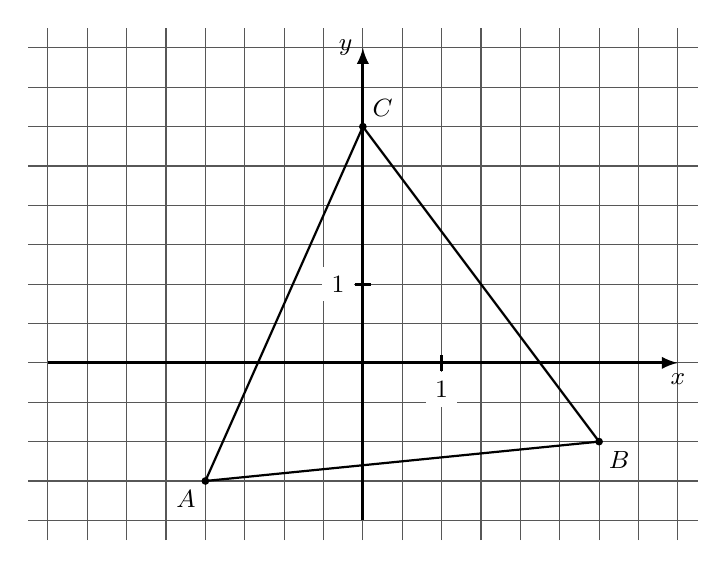
\begin{tikzpicture}[scale=1]
        \coordinate (A) at (-2, -1.5);
        \coordinate (B) at ( 3, -1);
        \coordinate (C) at ( 0,  3);
        \draw[thin, draw=black!66!white] (-4.25, -2.25) grid[xstep=5mm, ystep=5mm] (4.25, 4.25);
        \draw[line width=1.0pt, ->, >=latex] (-4, 0) -- (4, 0) node[below]{{\small$x$}};
        \draw[line width=1.0pt, ->, >=latex] (0, -2) -- (0, 4) node[left]{{\small$y$}};
        \fill (A) circle (1.4pt);
        \fill (B) circle (1.4pt);
        \fill (C) circle (1.4pt);
        \node[below left]  at (A) {{\small$A$}};
        \node[below right] at (B) {{\small$B$}};
        \node[above right] at (C) {{\small$C$}};
        \draw[line width=0.8pt] (A) -- (B) -- (C) -- cycle;
        \draw[line width=1.0] ([shift={(90:1mm)}]1, 0) -- ([shift={(270:1mm)}]1, 0) node[below, shape=rectangle, fill=white]{{\small$1$}};
        \draw[line width=1.0] ([shift={(0:1mm)}]0, 1) -- ([shift={(180:1mm)}]0, 1) node[left, shape=rectangle, fill=white]{{\small$1$}};
      \end{tikzpicture}
    \end{center}
  \fi
  \ifoutline\outline
    Benutze die Koordinaten der Eckpunkte\ldots
  \fi
  %\ifoutcome\outcome
  %\fi
\end{exercise}
